% Index of /design/

\section{Farben und Formen}
\label{sec:Farben und Formen}

\subsection{Farbgebung}
\label{subsec:Farbgebung}
\begin{figure}[H]
    \begin{center}
    		% GFX Trim left bottom right top
        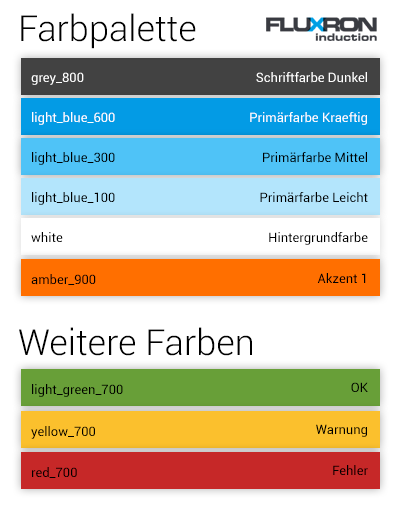
\includegraphics[trim=0 200 0 50,clip,scale=0.7]{uiux/res/basic_colors}
    \end{center}
    \caption{Grundlegende Farben der App}
\end{figure}
Die Farbgebung inspiriert sich am Logo der Firma Fluxron. Ein weisser Hintergrund, mit dunkelgrauer Schrift. Zudem wird ein simples aber aussagekräftiges Komplementärfarbschema zur Hervorhebung spezieller Elemente angewendet.

\subsection{Farben zur Statusanzeige}
\label{subsec:Farben zur Statusanzeige}
\begin{figure}[H]
    \begin{center}
    		% GFX Trim left bottom right top
        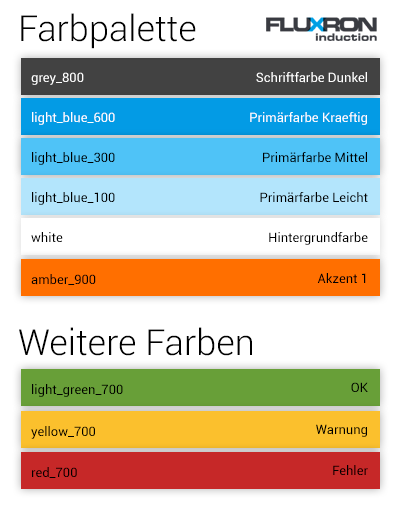
\includegraphics[trim=0 0 0 370,clip,scale=0.7]{uiux/res/basic_colors}
    \end{center}
    \caption{Farben zur Statusanzeige}
\end{figure}
Zur Anzeige von Statusinformationen wird ein klassiches Ampel-Farbschema angewendet. Dieses soll durch die Nutzung von Symbolen unterstützt werden. Diese Farben sollten nur für kleine Flächen genutzt werden.